\documentclass{report}

\usepackage{listings}
\usepackage{url}
\usepackage{color}
\usepackage[utf8x]{inputenc}
\usepackage{lmodern,textcomp}
\usepackage{graphicx}
\usepackage{minitoc}


%\usepackage[Lenny]{sty/fncychapleo}

\definecolor{light-gray}{gray}{0.97}
\lstset{numbers=left,
  basicstyle=\small,
  numberstyle=\tiny, 
  breaklines=true,
  backgroundcolor=\color{light-gray},
  numbersep=5pt,
  xleftmargin=.25in,
  xrightmargin=.25in,
  keywordstyle=\color[rgb]{0,0,1},
  commentstyle=\color[rgb]{0.133,0.545,0.133},
  stringstyle=\color[rgb]{0.627,0.126,0.941},}

\title{How are we tracked in our everyday life ?}
\author{Martin Trigaux}
\date{\today}

\begin{document}

\maketitle

\dominitoc

\section*{Introduction}

\part{State of the art}
\label{chap:general}

\chapter{Phone}

\chapter{RFID}

\chapter{Wifi}

\chapter{Other}

\part{Android}
\label{chap:android}
\minitoc

\chapter{Localization under Android}

\section*{Introduction}
The localization of the user is a key function under Android. It allows to directly show the part of the map where the user is on Google  Maps, to display adds for shops close to you, to find the weather forecast of the area you are, to gives statistical information of the country usage of an application... Many applications use it and it is often an asked permission at the installation.\\

This chapter will explain how to 

\section{Available techniques}
Depending of the state of the phone, several techniques can be used to locate an Android device.

\subsection{GPS}
The GPS, for Global Positioning System is a technology based on satellites trilateration. GPS satellites are navigating around the earth in a way to maximize the number of visible satellite anywhere at any time. There is currently 31 working satellites in orbit.
The location-aware device is equiped with a GPS receiver ship. This receiver will retrieve broadcasted messages from the reachable satellites. The messages contains :
\begin{itemize}
\item the time the message was transmitted
\item precise orbital information (the ephemeris)
\item the general system health and rough orbits of all GPS satellites (the almanac)
\end{itemize}

Trilateration is used based on the received messages. If theoriaclly, three satellites are enough, at least four is requiered to avoid clock desynchronisation errors (at the speed of light, even an small clock error can lead to huge error).\\

The accuracy of this method depends of the surrounding of the user. In clear sight, the accuracy will be of a few meters but will degrade if the receiver is surrounded by high building or inside a dense forest.

\subsection{Wireless access point}
Each wireless access point has a unique BSSID such as \texttt{00:19:70:31:4A:87}. If the wireless is turned on, the device can retrieve the surrounding access points. Assuming the geographical coordinates of the access point are known, it is possible to have a estimation of the location of the user by trilateration.\\

The advantage of this method is that for an accuracy of about 100 meter, the localization is faster than using GPS, consumes less battery power than a GPS receiver ship and doesn't have other geographical requierement than being surrounded by at least one access point.\\

The collect method used by Google is explained below.

\subsection{Cell tower}
Similar as for the location using wireless access points, a phone can be located using trilateration based on the surrounding cell towers. On the GSM network, a cell tower is characterized by a Cell-ID and the Location Area Code.\\



\subsection{Android API}
When an application wants to locate the device position, the Android system provides some high level methods to use the available technologies listed above. Getting a user location in Android works by means of callback. A \texttt{LocationListener} is defined and will react to event such as \texttt{onLocationChanged} or \texttt{onProviderEnabled}. On the relevent event, the callback function is executed and the location retrieved\footnote{ \url{http://developer.android.com/guide/topics/location/obtaining-user-location.html#Updates}}.

\lstset{language=Java}
\begin{lstlisting}[label=location-base,caption=Code from Android developers guide]
// Acquire a reference to the system Location Manager
LocationManager locationManager = (LocationManager) this.getSystemService(Context.LOCATION_SERVICE);

// Define a listener that responds to location updates
LocationListener locationListener = new LocationListener() {
    public void onLocationChanged(Location location) {
      // Called when a new location is found by the network location provider.
      makeUseOfNewLocation(location);
    }

    public void onStatusChanged(String provider, int status, Bundle extras) {}

    public void onProviderEnabled(String provider) {}

    public void onProviderDisabled(String provider) {}
  };

// Register the listener with the Location Manager to receive location updates
locationManager.requestLocationUpdates(LocationManager.NETWORK_PROVIDER, 0, 0, locationListener);
\end{lstlisting}
  
At any moment, a user can request the last known location using the following code

\begin{lstlisting}[label=getLastKnown,caption=Get the last recorded location]
LocationProvider locationProvider = LocationManager.NETWORK_PROVIDER;
// Or use LocationManager.GPS_PROVIDER

Location lastKnownLocation = locationManager.getLastKnownLocation(locationProvider);
\end{lstlisting}

The provider \texttt{GPS\_PROVIDER}  or \texttt{NETWORK\_PROVIDER} allows to choose the source of the location. The GPS is used in the first case and an hybrid method using both wireless and cell tower location in the second.

\section{Access points and cells databases}
To locate a device using the \texttt{NETWORK\_PROVIDER}, the system needs to access to a database mapping the geographical coordinates of the requested access points and GSM cell tower.\\

SkyHook was one of the first database locating wireless access points and developed an SDK to query the location of a user .
The information are collected by war driving in North America, Western Europe and some Asian countries\footnote{\url{http://www.skyhookwireless.com/location-technology/coverage.php}}.

Compagnies have quickly understood the interest of having such database.
While Apple was, at first, using ShyHook, it has now developped its own database. Google is also independent and has created its own database.

\subsection{Collect method}
The Google Location Server is constructed based on two factor :
\begin{itemize}
\item Google Cars
\item Crowdsourcing
\end{itemize}

The Google Cars are mainly used to take pictures to illustrate the service Google Street View. In addition to that, the cars are also wardriving.  Having a GPS module on the car and driving almost all over the world, it was a good oportunity to constitute a very accurate database.\\

In May 2010, Google admited to German authorities having collected more than what it was supposed to. In addition to access point BSSID, it had ``been mistakenly collecting samples of payload data from open networks''. These data chunks could include parts of an email, text or photograph or even the website someone may be viewing\footnote{\url{http://news.techeye.net/security/google-admits-it-sniffed-out-peoples-data}}. In reaction, the data collected data were asked to be deleted and the CNIL (independent French administrative authority) fined Google with €100.000\footnote{http://www.bbc.co.uk/news/technology-12809076}.\\

As most Android devices are equiped with a GPS receiver, crowdsourcing the collect is also possible. When an Android device use the Google database to request a location, data are also transmited to Google servers. This way, the database of wireless access points and cell tower is always up to date.\footnote{\url{http://franciscokattan.com/2010/02/06/dynamic-cell-id-clever-way-to-block-google-but-will-it-backfire/}}

\subsection{Analysis of requests made}

When a location is requested on an Android device, the system sends an encrypted request to the Google's location servers. The Google's servers reply to the request with the location of surrounding GSM cell towers and access points.\\

In the Android internal memory are stored a number of previous cell and access points locations. This allows to locate the user quickly, even when he is not connected to internet. This local cache file is stored in the folder \texttt{/data/data/com.google.android.location/files} in the files \texttt{cache.wifi} and \texttt{cache.cell}. Each entries in the cache file is linked with a timestamp representing the date of the retrieval as seen in figure \ref{fig:locmap}. Only the 50 last cells and 200 access points have been observed as stored in the cache files. A python script as been developped\footnote{\url{https://github.com/packetlss/android-locdump}} to parse the content of these two files and output a GPS trace representing the approximate deplacement of the device. A root access to the phone is however requiered to access these files (which most of the time requiere system manipulation and void the warranty). Also this cache folder is only composed when the \emph{Use wireless networks} option is enabled in the Android settings (often requiered by apps such as Google Maps). When the option is disabled, the cache files are deleted.

\begin{figure}[h]
  \centering
  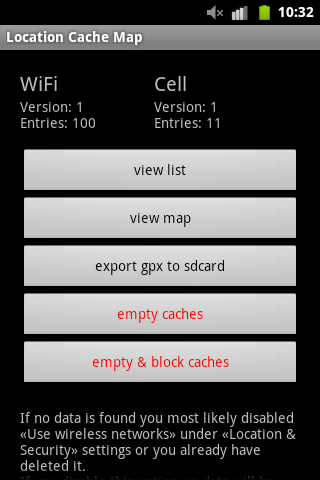
\includegraphics[width=4cm]{includes/cache1.png}
  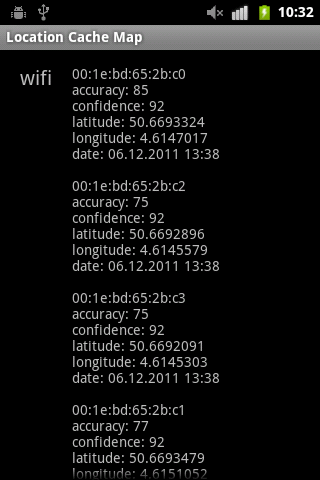
\includegraphics[width=4cm]{includes/cache2.png}
  \caption{Captures from the application Location Cache by Remy Demy}
  \label{fig:locmap}
\end{figure}


\subsubsection{Personal research}

To understand the content of the requests, two analysis have been made. The first one to ensure the location informations are stored only in the two cache folders and that they are deleted once the option is disabled. The second one is an analysis of the volume of transmitted data correlated to the number of entries added in cache. To realise the analysis, the applications present in the appendix X have been used.\\

The first analysis was done in two experiments. To ensure that the location information is only stored inside the cache files, the following experiment was done :
\begin{enumerate}
\item Make a dump of the internal memory
\item Request a location update
\item Make a dump of the internal memory
\item Compare the two dumps
\end{enumerate}

The analysis reveal that, with the exception of meaningless system files, only the database cache files have been modified.\\

To ensure the information is deleted from the system when the \emph{Use wireless networks} option is opt out, the following experiment was done.

\begin{enumerate}
\item Make a dump of the internal memory
\item Disable the \emph{Use wireless networks} option
\item Make a dump of the internal memory
\item Compare the two dumps
\end{enumerate}

The analysis reveal that, with the exception of some irrelevant system files (battery state...) modified, the database cache and Google Maps cache have been deleted.\\

The second analysis used tcpdump to corelate a request with the content of the cache files.

\begin{enumerate}
\item Start in \emph{blank state}\footnote{\emph{Blank state} : wireless turned off, empty location cache, location permission turned off, no process requiering the location running such as Google Maps}
\item Start tcpdump
\item Activate the wireless
\item Request a location with the application \emph{LocateMe}
\item Stop tcpdump once a location received
\end{enumerate}

The analysis compared the size of the data transmitted with the number of cells and access points stored in the cache folder.\\

\begin{figure}[h]
  \hspace*{-2cm}
  \centering
  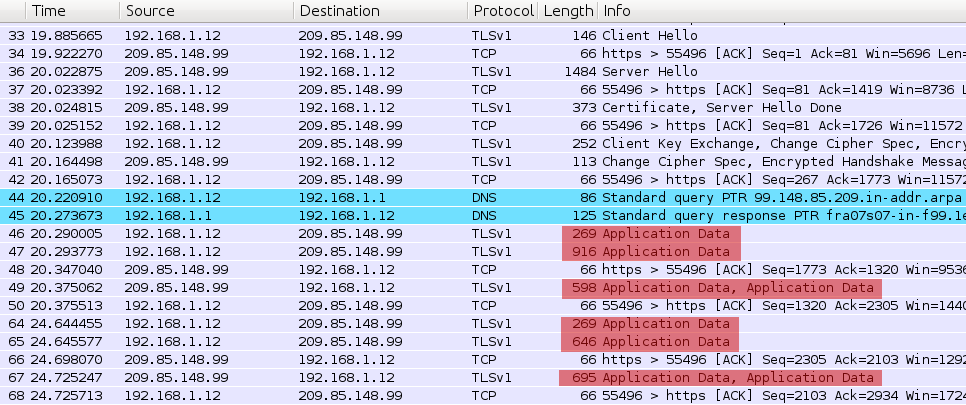
\includegraphics[width=17cm]{includes/trace2.png}
  \caption{Example of tcpdump capture while a location request}
  \label{fig:tcpdump}
\end{figure}

After observation, the following pattern was derivated :
\begin{itemize}
\item Two requests are made, one for the cells, one for the wifi.
\item The first paquets contains always 269 bytes.
\item The uploaded data size is bigger than the downloaded.
\item The size of the downloaded data is directly linked to the number of entries in the cache files.
\end{itemize}


\subsubsection{Research of Samy Kamkar}

To reply to privacy concerns, Google ensured ``The location information sent to Google servers when users opt in to location services on Android is anonymized and stored in the aggregate and is not tied or traceable to a specific user''\footnote{Alan Davidson, director of public policy at Google \url{https://docs.google.com/viewer?a=v&pid=explorer&chrome=true&srcid=0BwxyRPFduTN2NmI2NGVjMWUtZDg0NC00NGI5LWJlYTctNmI4MGQ2YmIzYzUz&hl=en}}.\\

\begin{figure}[h]
  \hspace*{-1cm}
  \centering
  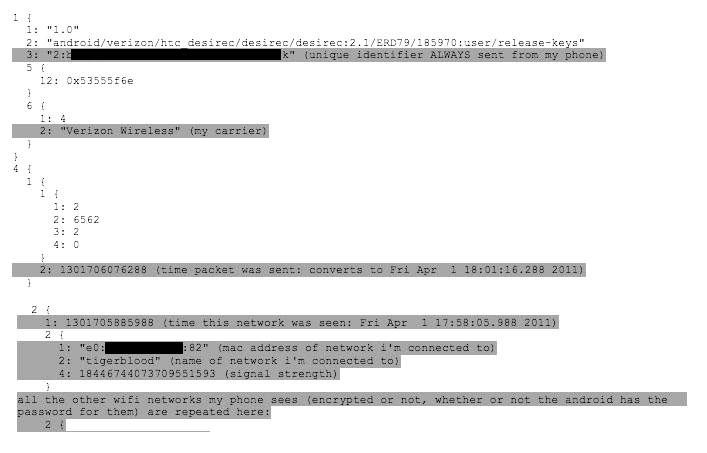
\includegraphics[width=15cm]{includes/reqdecode.jpg}
  \caption{Decrypted request content reveal to CNet by Samy Kamkar}
  \label{fig:reqdecode}
\end{figure}

Samy Kamkar, a security researcher, succeeded to decrypt the request made to Google server and realized a unique identifier is always sent from its phone (see figure \ref{fig:reqdecode}).\footnote{\url{http://news.cnet.com/8301-31921_3-20056657-281.html}}. If this string does not directly reveal the identity of the phone owner, it is however possible to tied the string to a specific user and then trace him. This string is contained inside the file \texttt{/data/data/com.google.android.location/files/gls.platform.key} and it is renewed every time the \emph{Use wireless networks} option is toggled. If it is relatively easy to change this value, we can imagine that very few users will apply this manipulation regulary.

\subsection{\_nomap}

In November 2011, in reaction to critiques about the automatic collect of data that some consider as private, Google created a way to opt out recording of its access point. The proposition of Google is to end the ESSID of the wireless access point with \texttt{\_nomap}. The next time it will be scanned by a Google Cars or an Android device, the access point will be removed from the database. Google hopes than over time, the \texttt{\_nomap} string will be adopted by other location providers.\footnote{\url{http://googleblog.blogspot.com/2011/11/greater-choice-for-wireless-access.html}}\\

This proposition was received with much skepticism and critiques. The main complain was the need of an action from the user to explicitely opt out its access point while people wanted a way to explicitely opt in instead. Many people that are consered by privacy issues do not have enough computers knowledge to modify its access point name.

\chapter{Security under Android}
\section{Permissions}

\section{Software}

\part{Camera}

\tableofcontents

\end{document}
